Having successfully stabilised prototype bicycle...

\begin{figure}[H]
	\begin{subfigure}{0.475\textwidth}
	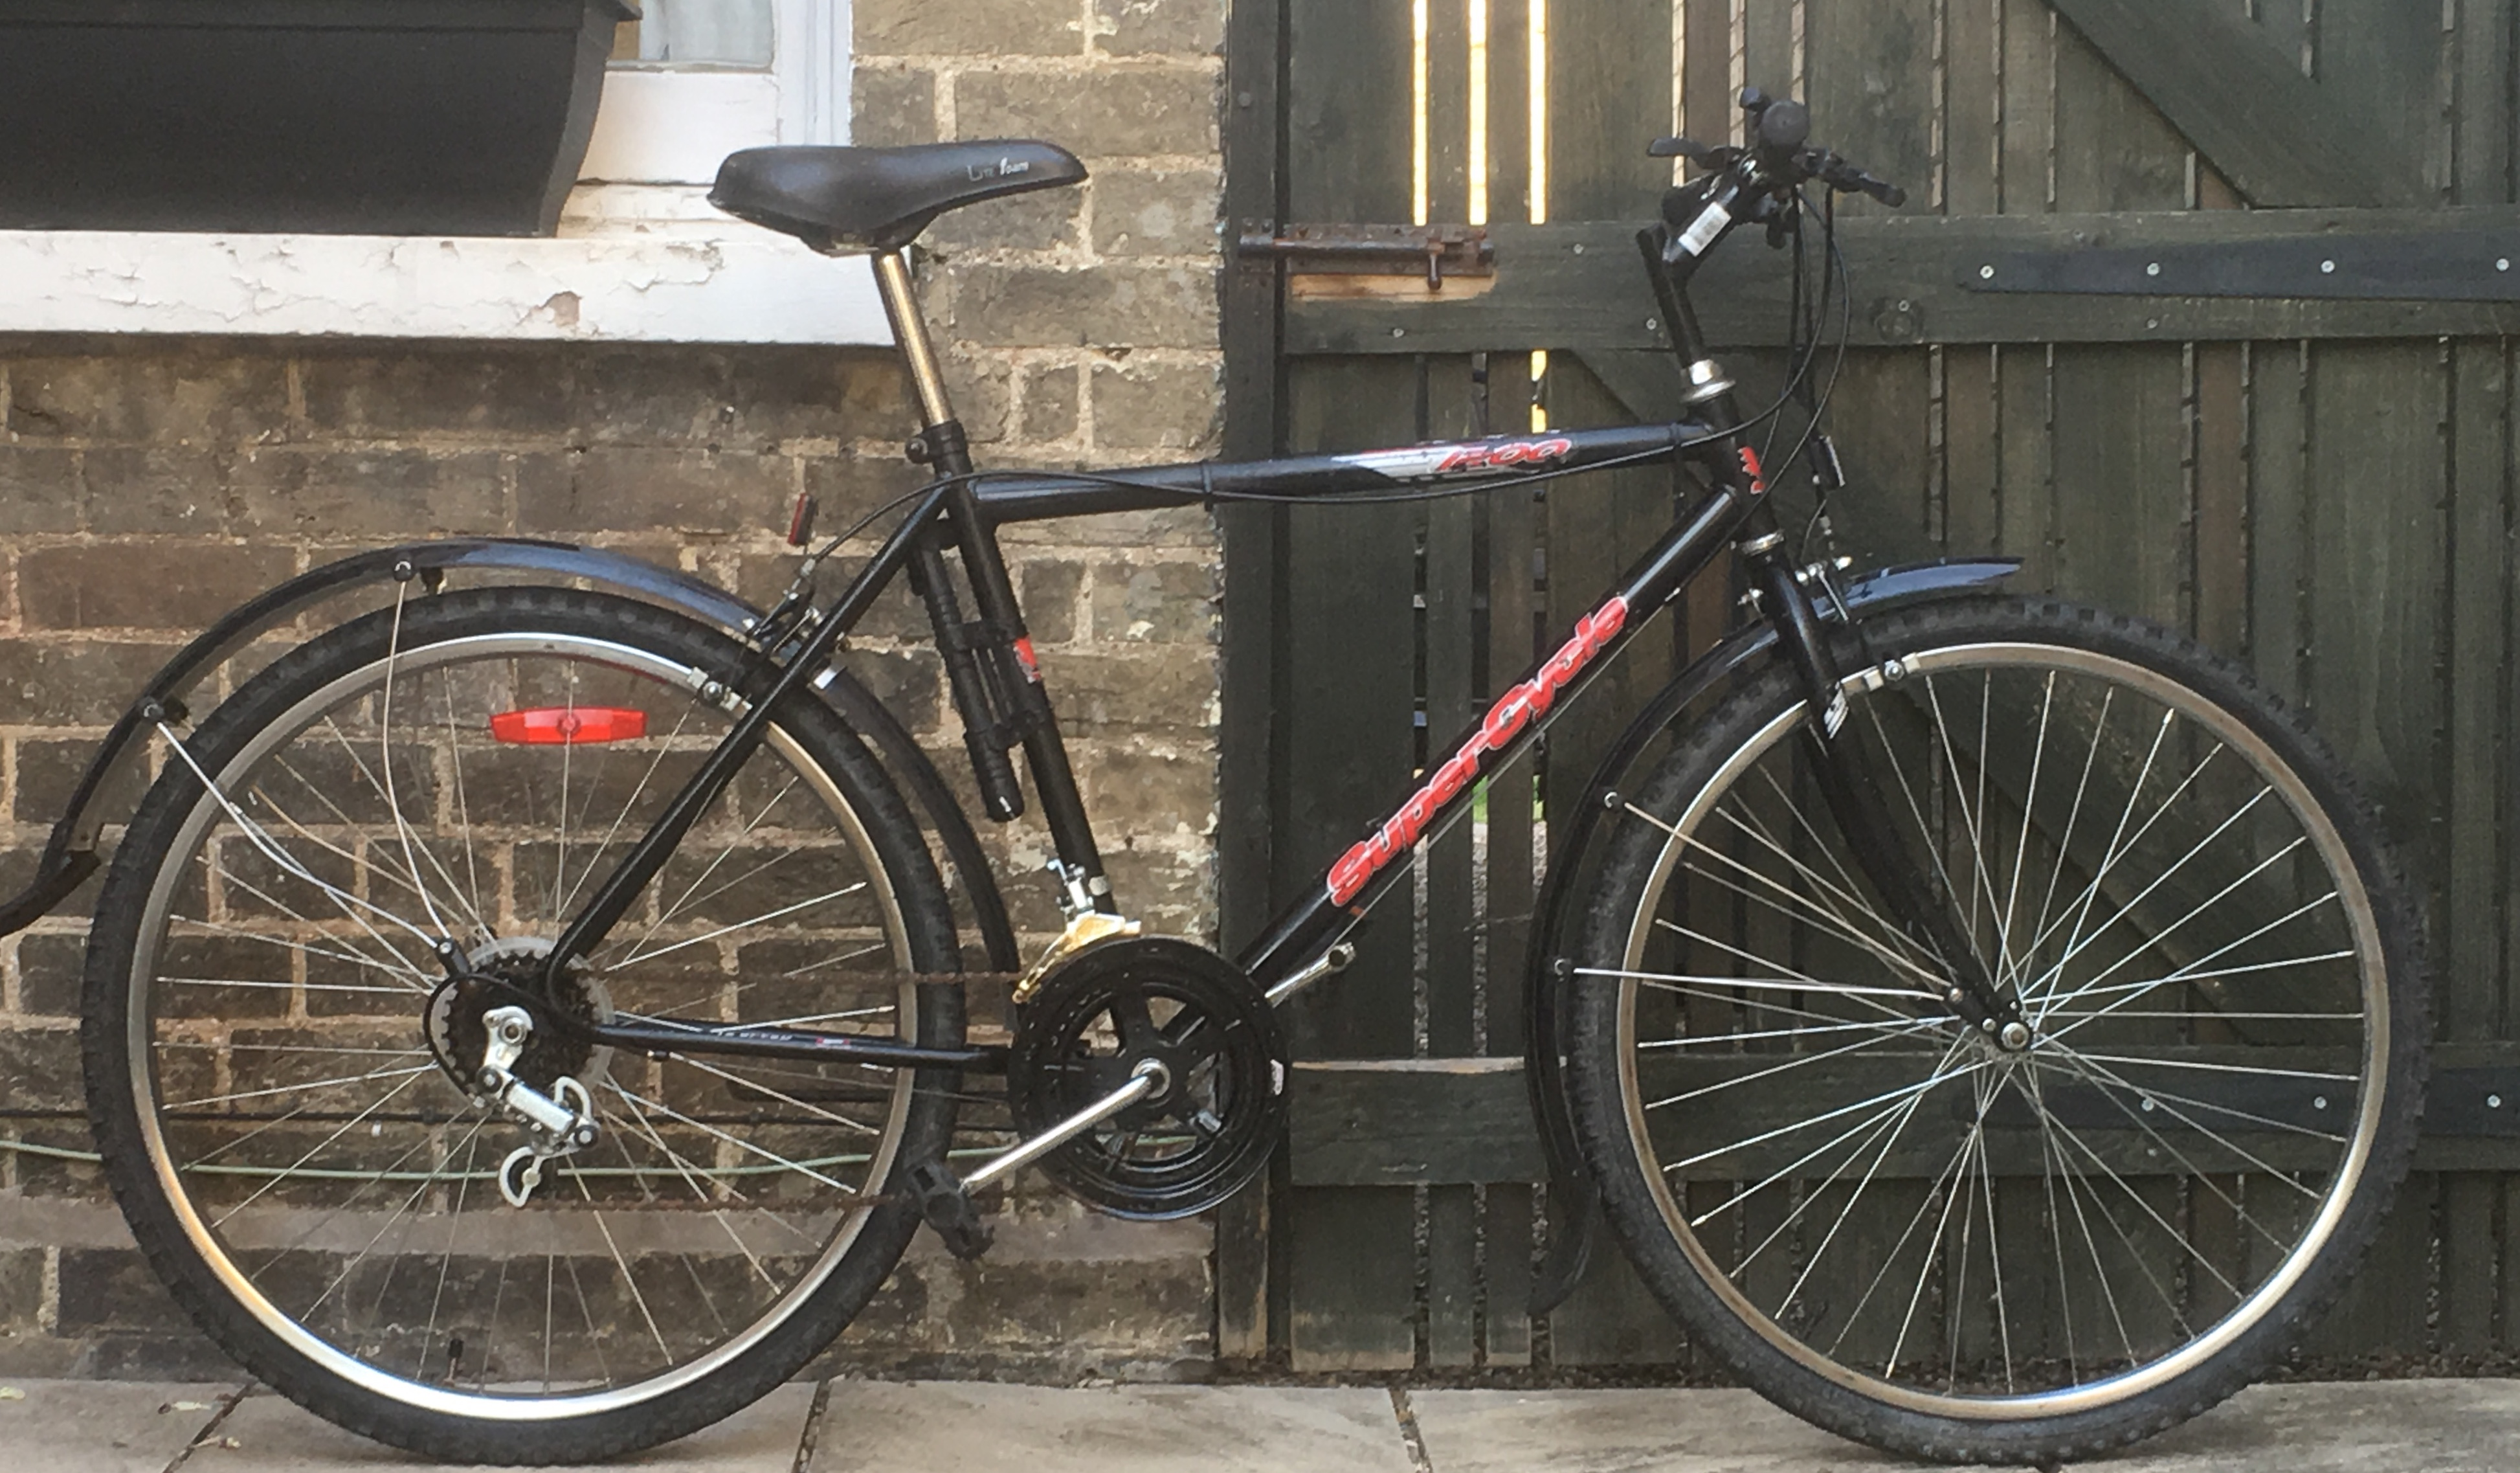
\includegraphics[scale=0.06]{FSBike}
	\caption{Unmodified Form}
	\end{subfigure} \hfill
	\begin{subfigure}{0.475\textwidth}
	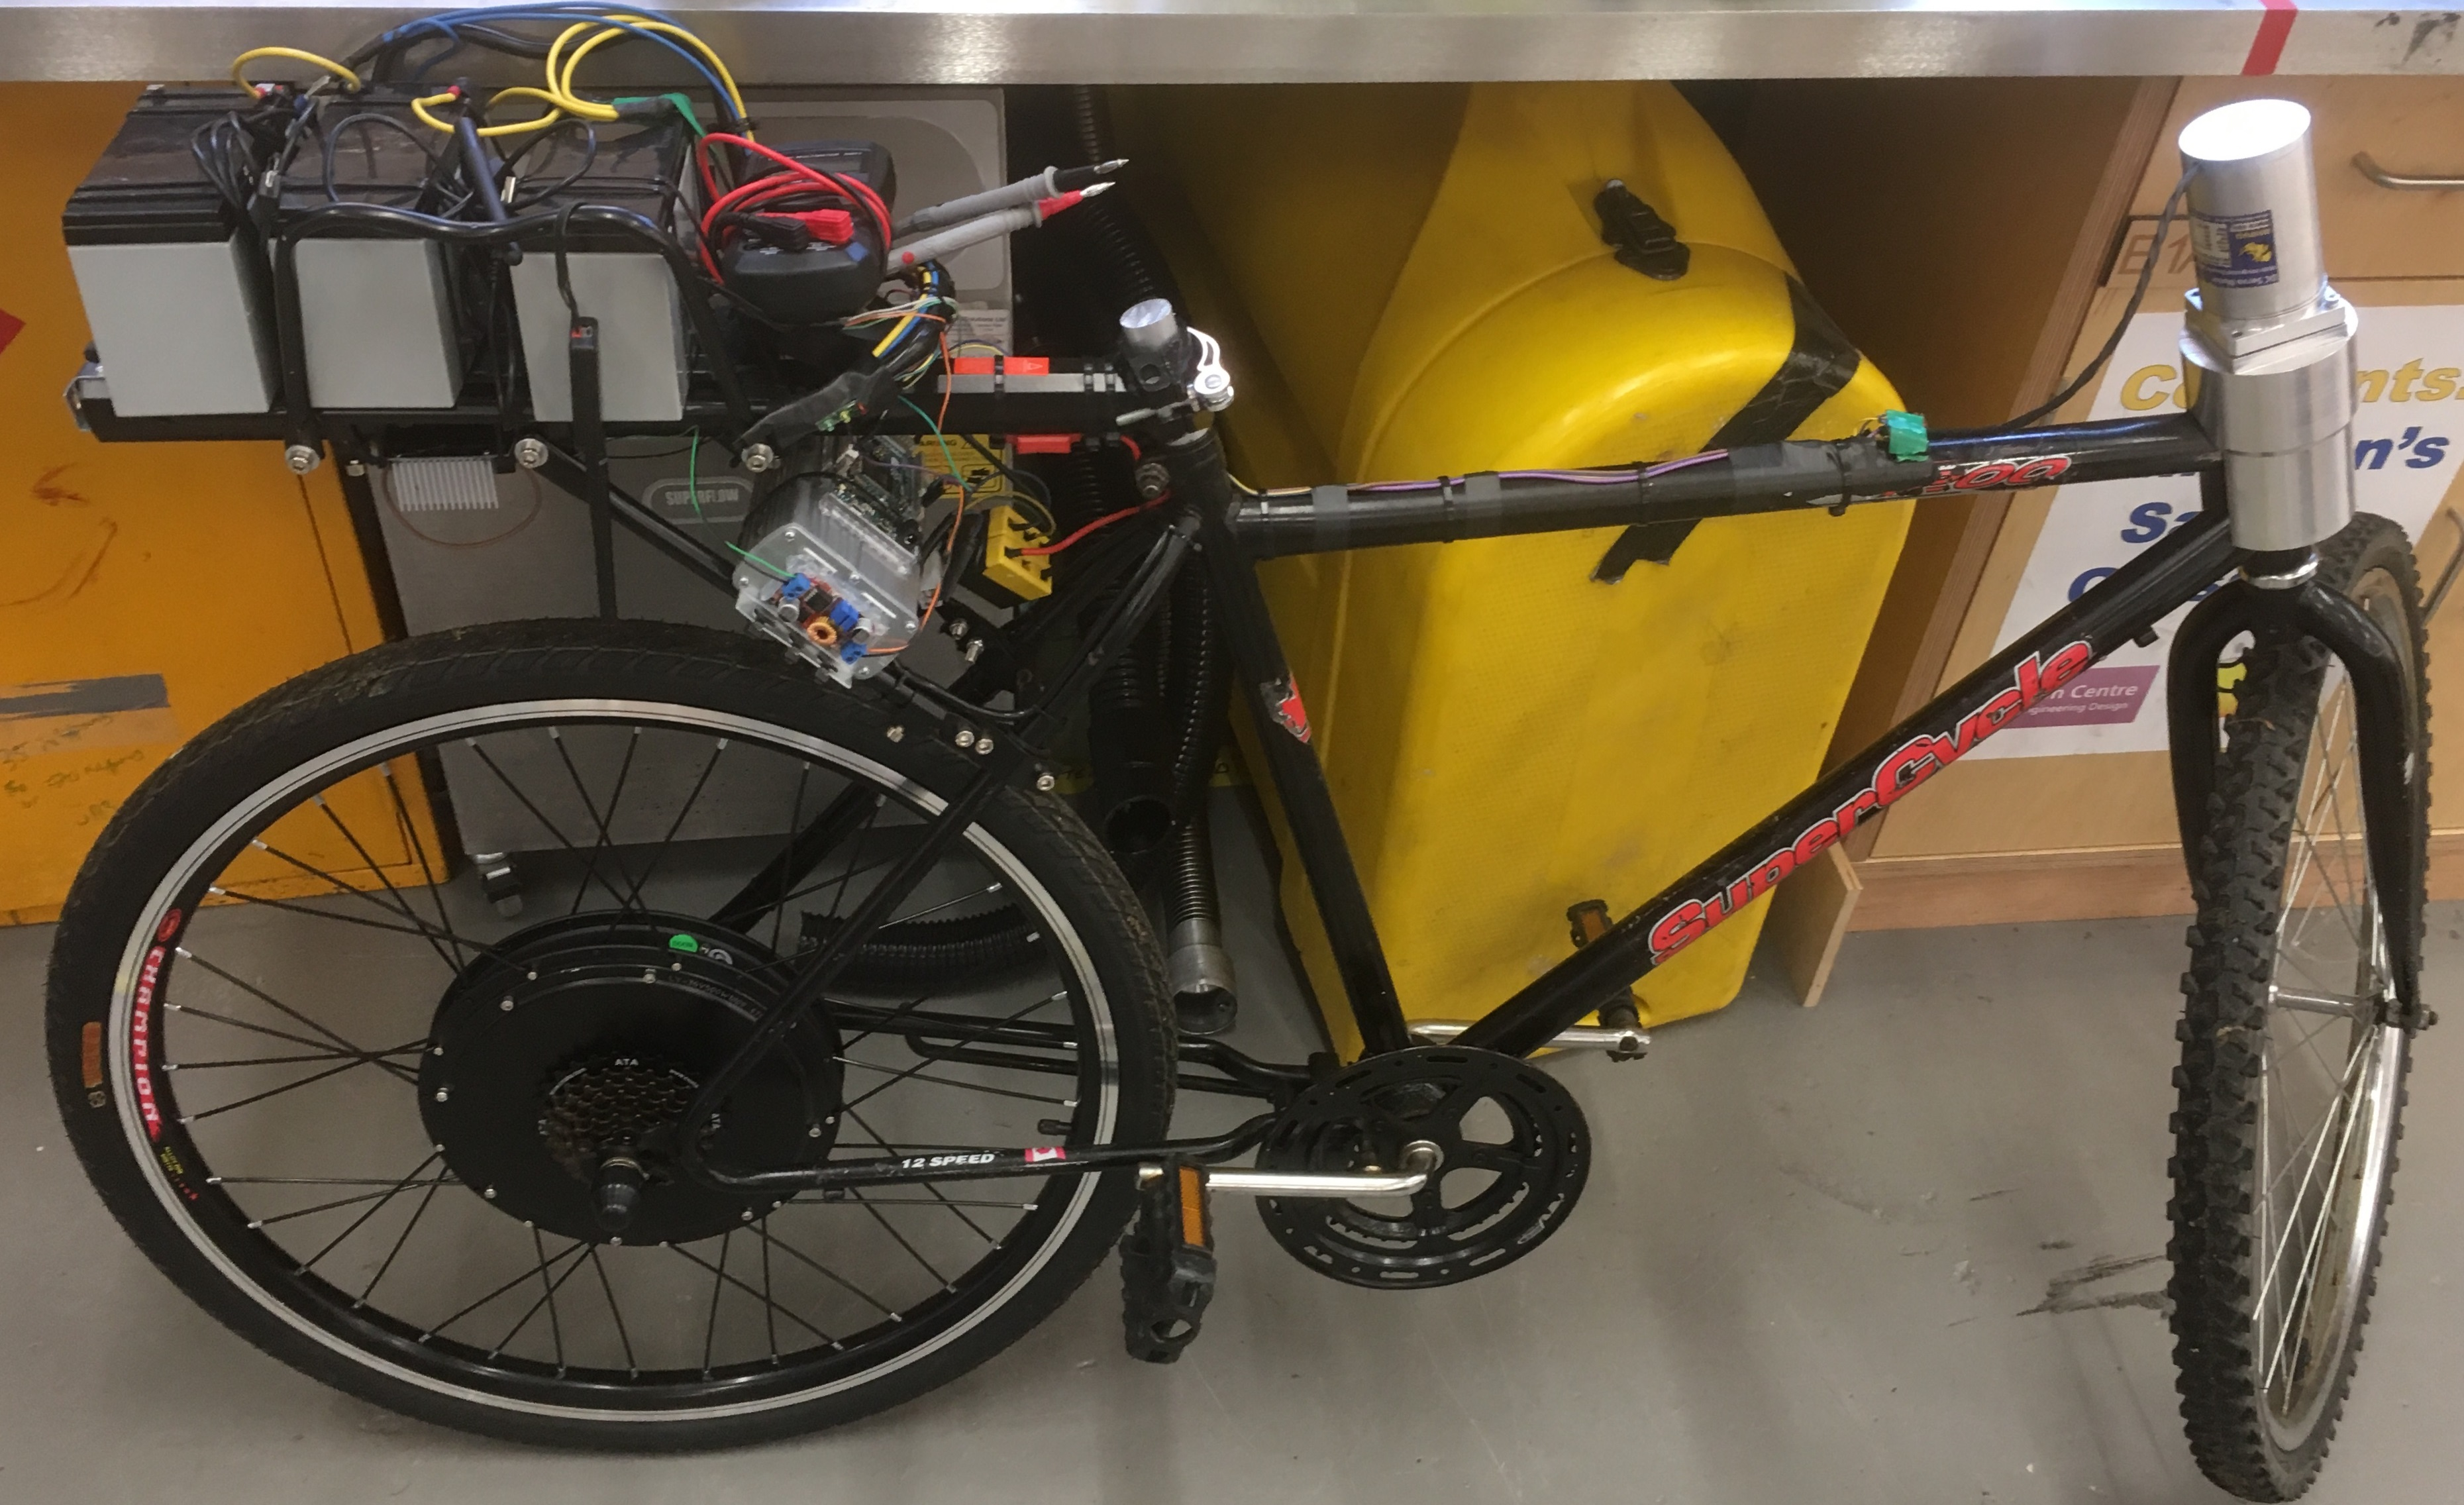
\includegraphics[scale=0.06]{FSBikeMod}
	\caption{After Modification}
	\end{subfigure}
	\caption{Full-Scale Bicycle Before and After Modification}
\end{figure}

\subsection{Hardware}

Arduino (32-bit instead of 8-bit) as controller, why particular servo, servo mounting design, battery, voltage regulators, drive motor, motor controller disassembly, etc. 

\newpage
\null
\vfill
\begin{figure}[H]
	\centering
	\begin{subfigure}[t]{0.475\textwidth}
		\centering
		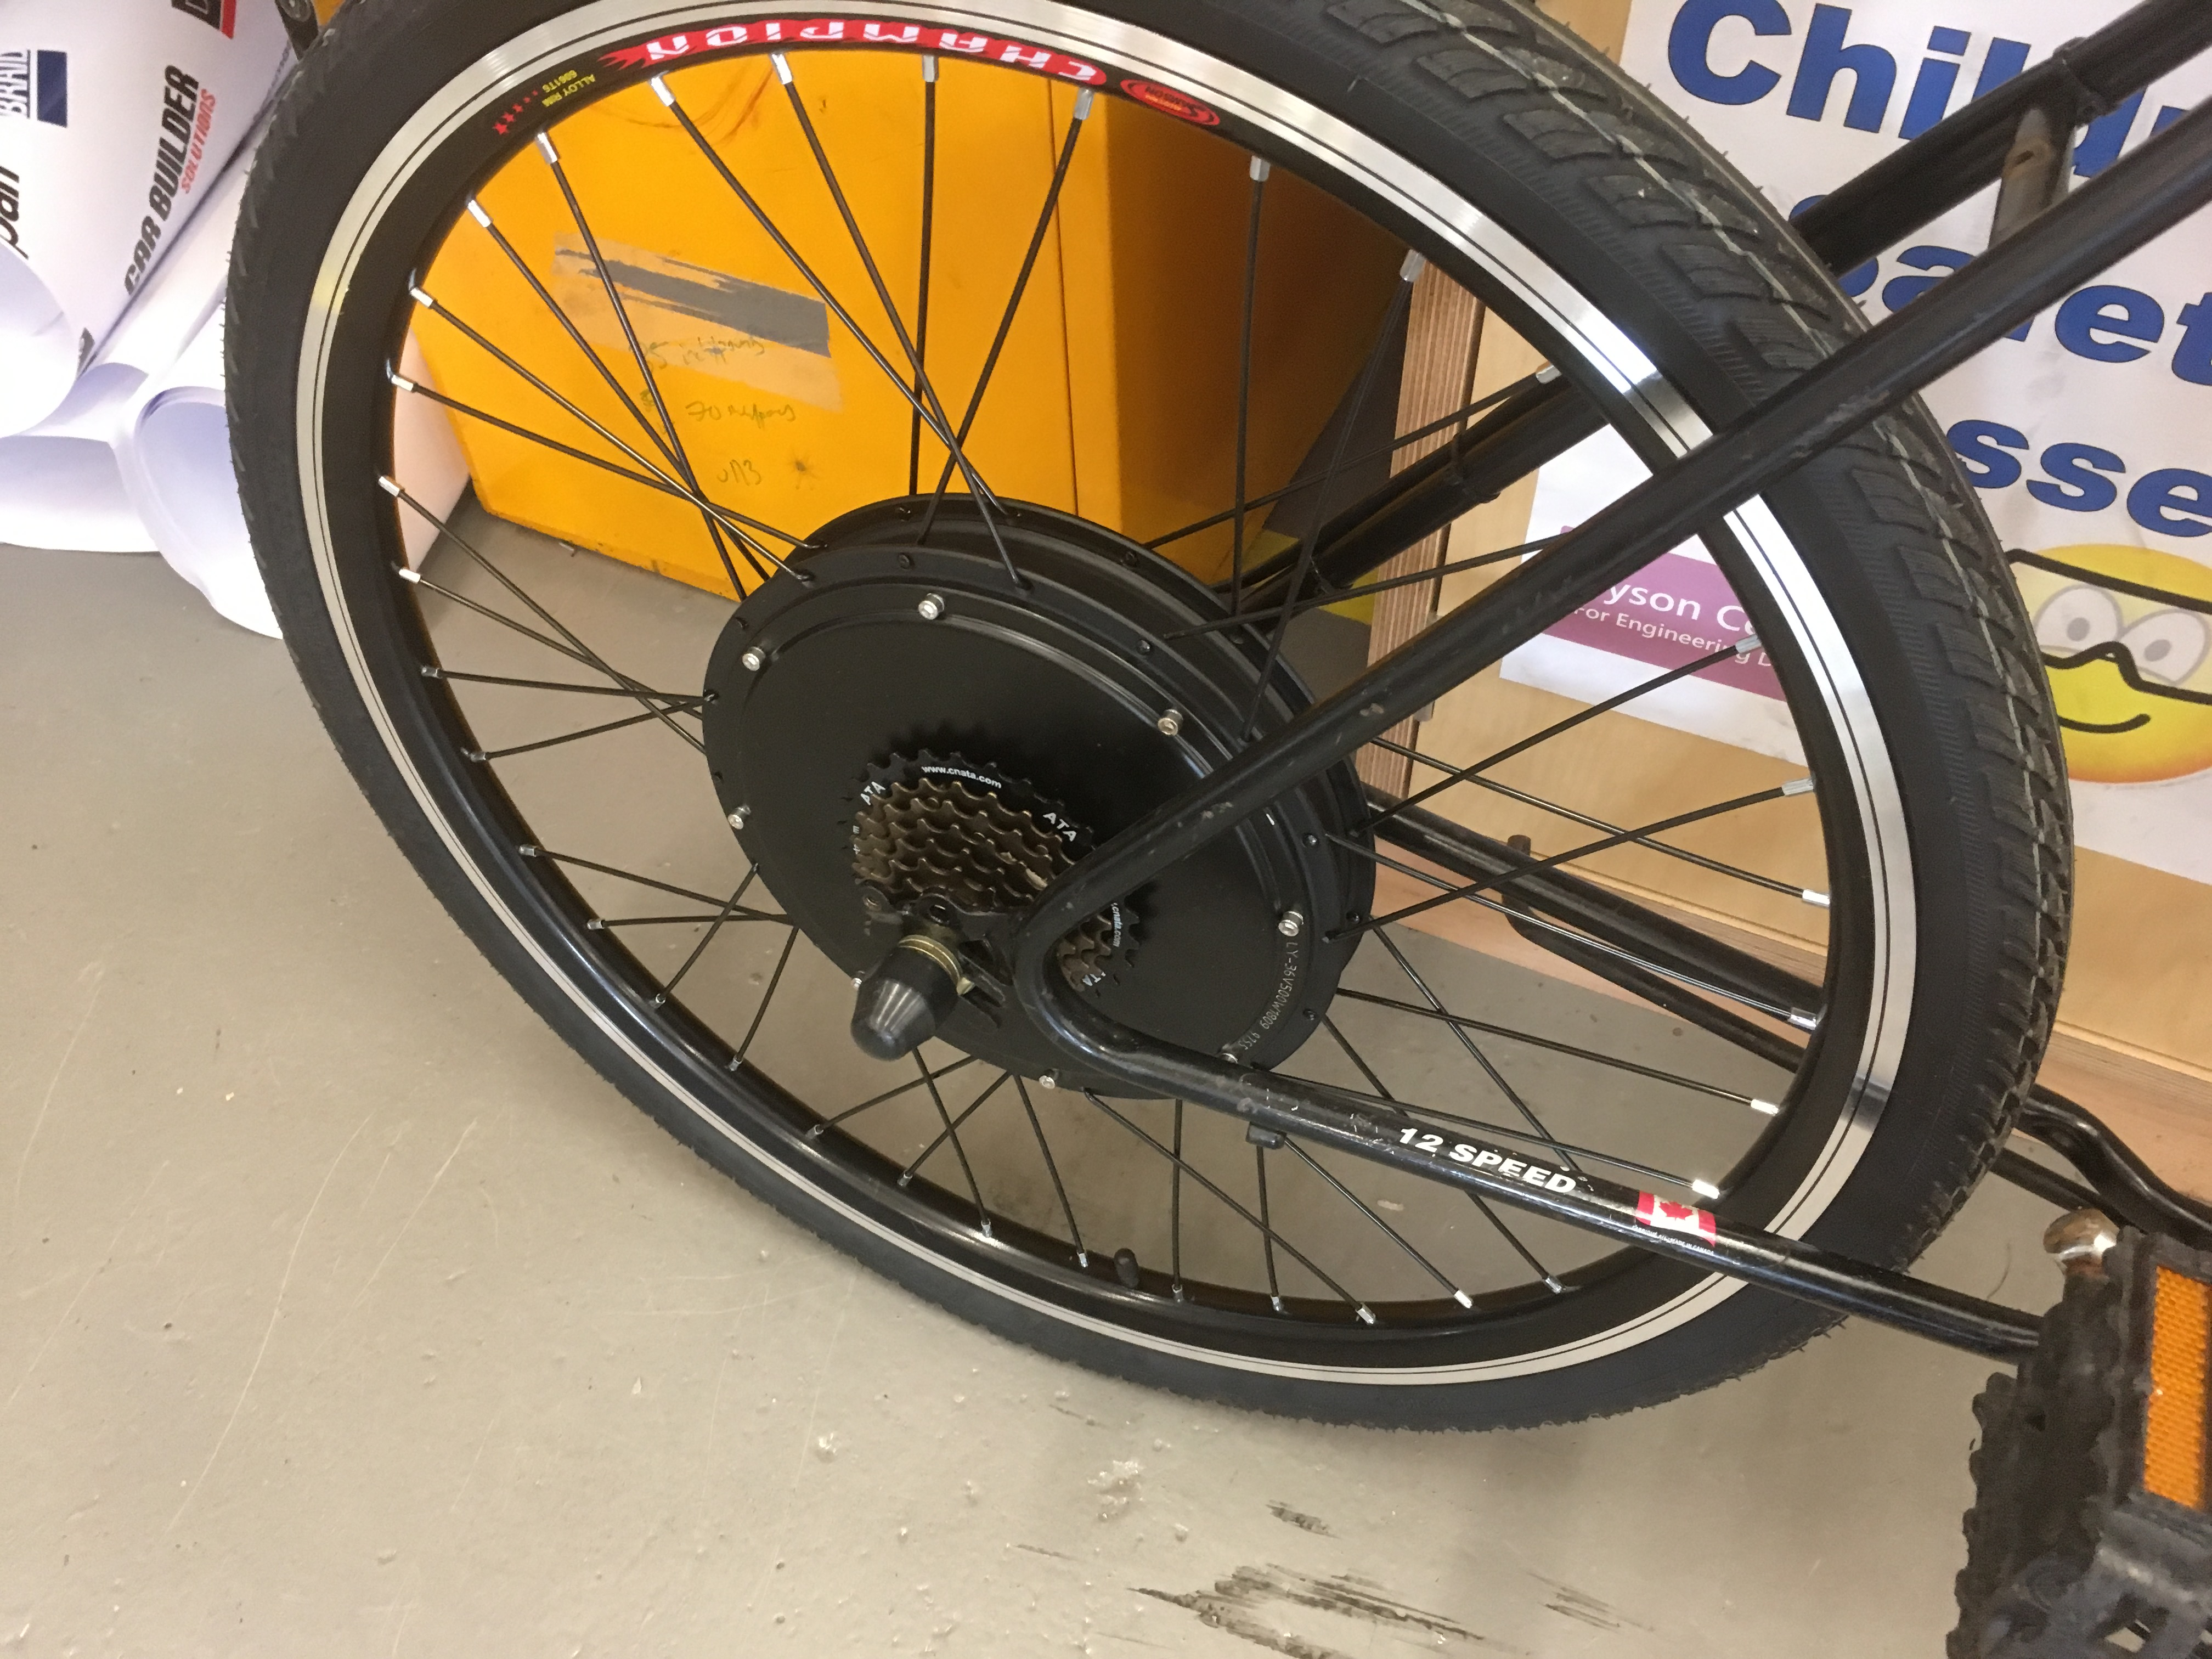
\includegraphics[width=\textwidth]{fsDrive}
		\caption{Rear Drive Motor}
		\end{subfigure}
	\hfill
	\begin{subfigure}[t]{0.475\textwidth}  
		\centering 
		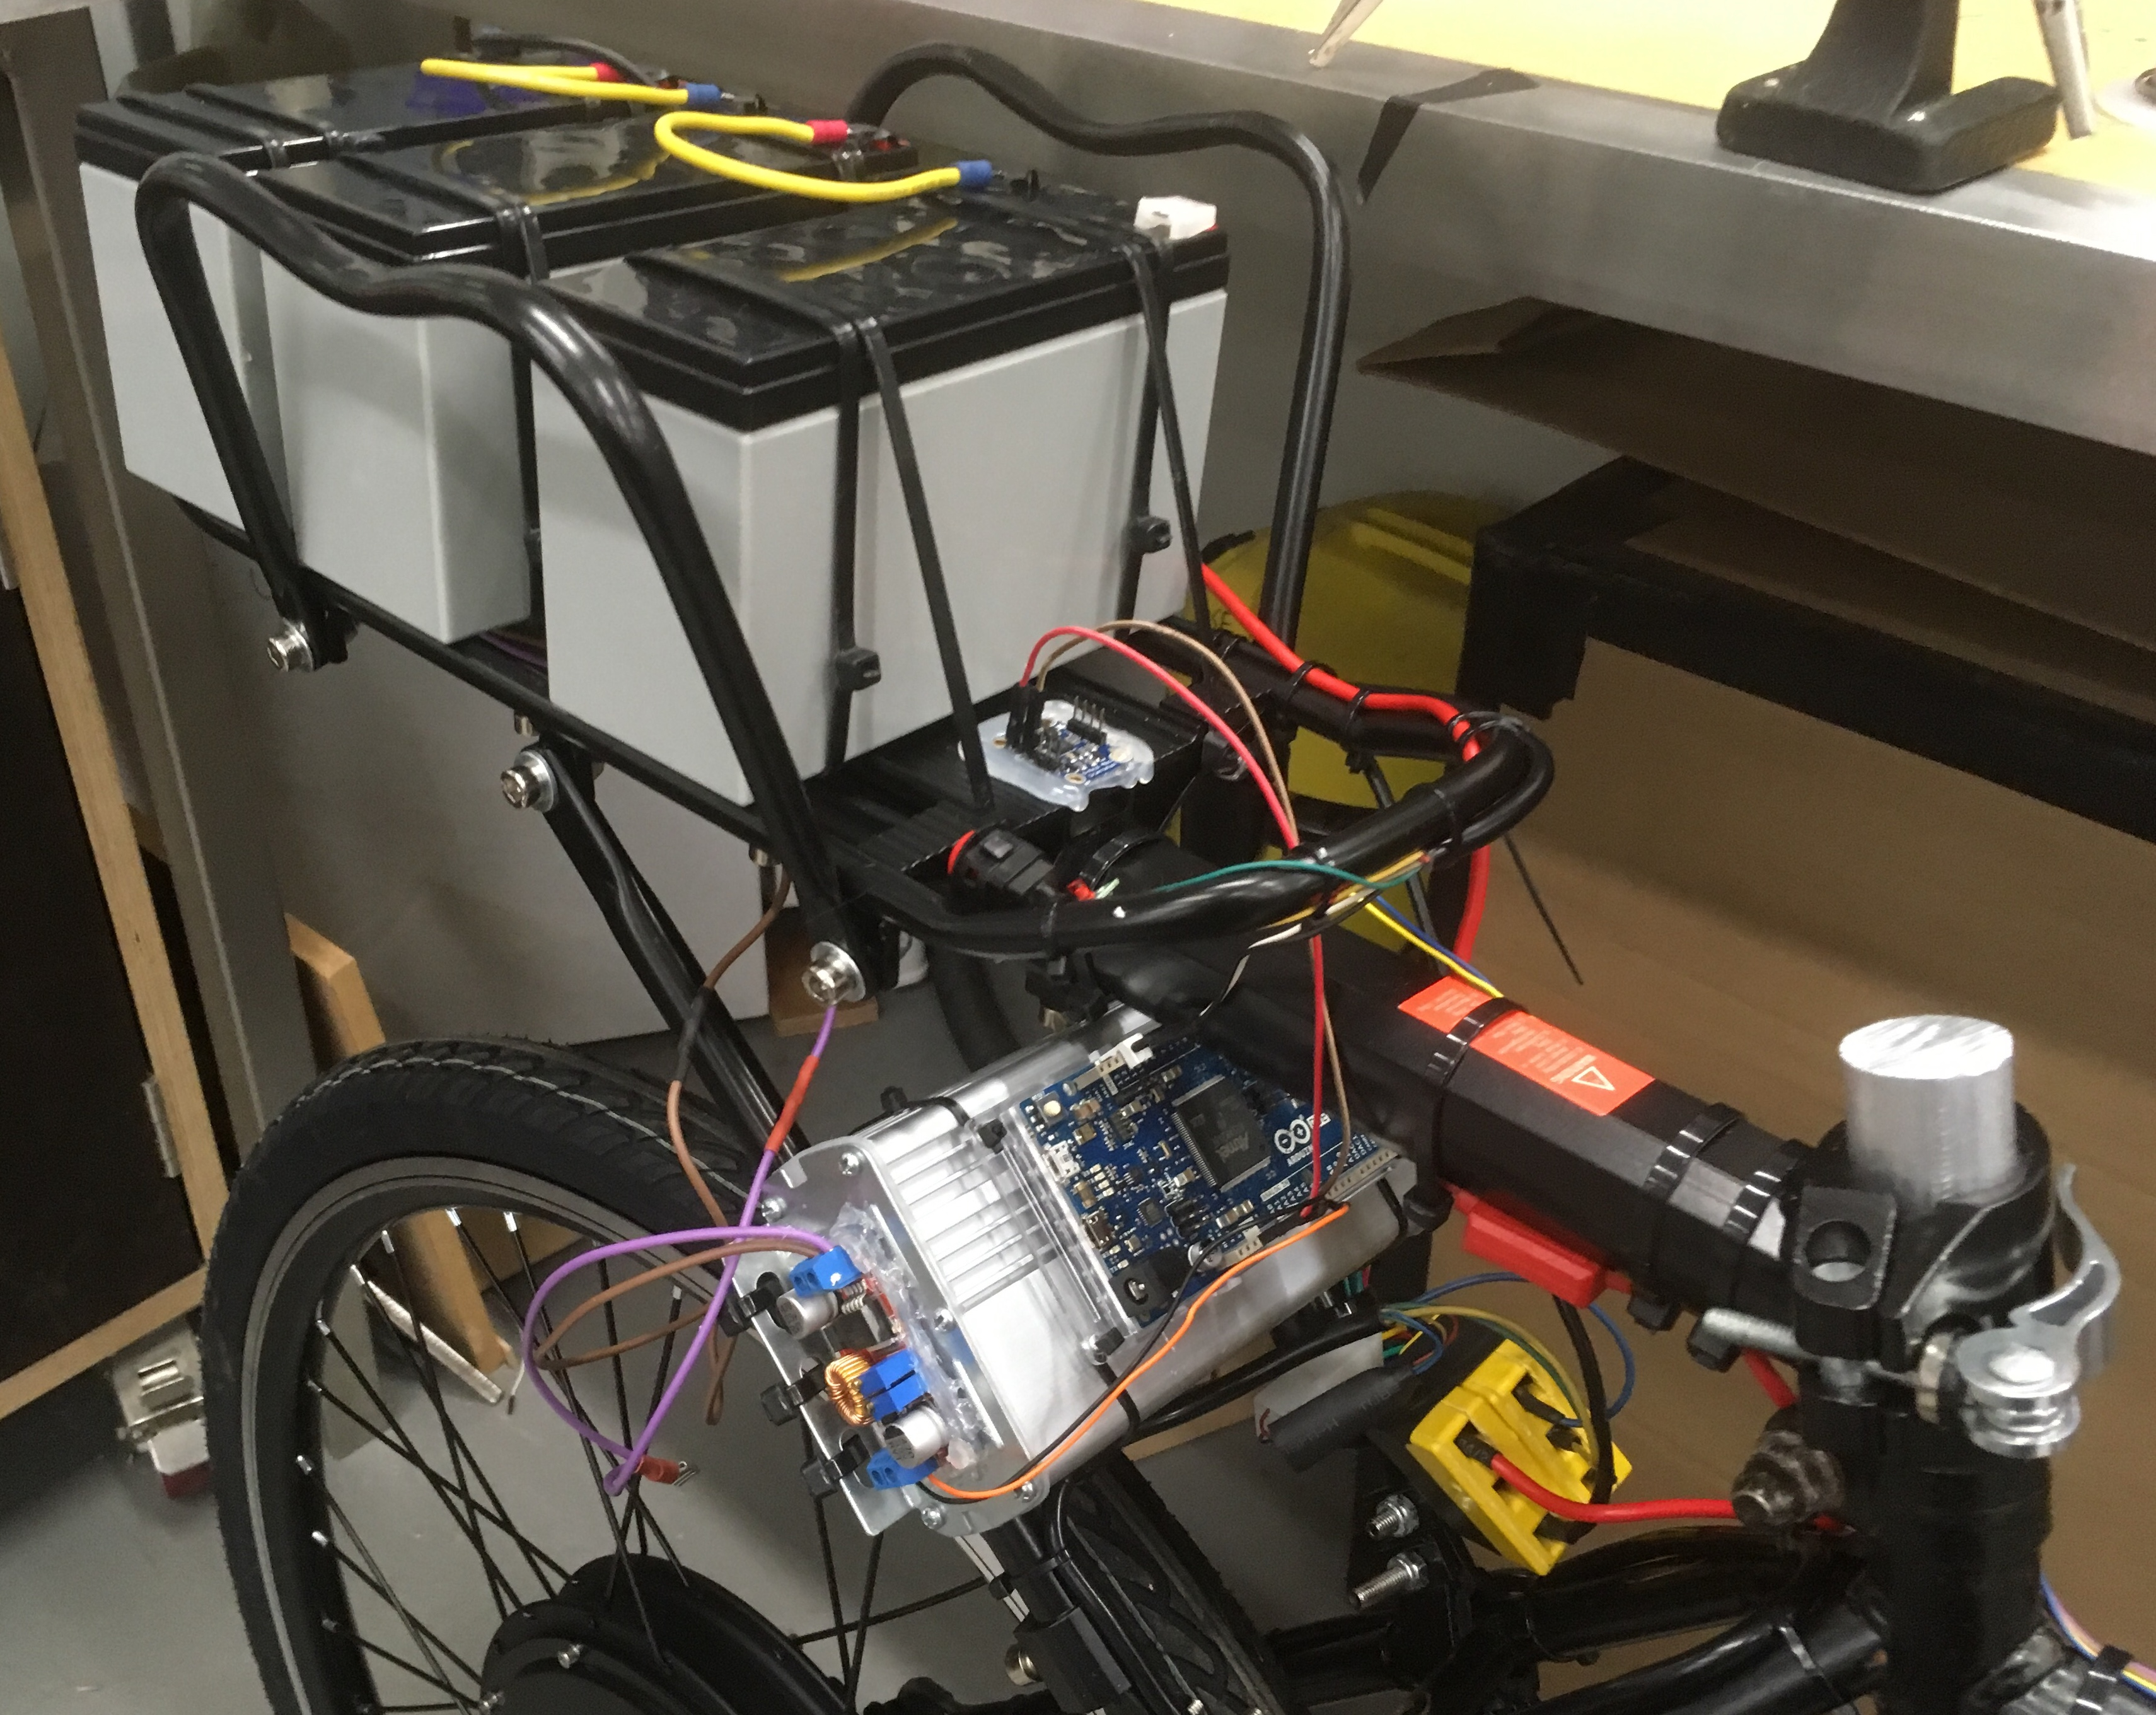
\includegraphics[width=\textwidth]{fsRear}
		\caption{Power and Control Section}
	\end{subfigure}
	\vskip\baselineskip
	\begin{subfigure}[t]{0.475\textwidth}   
		\centering 
		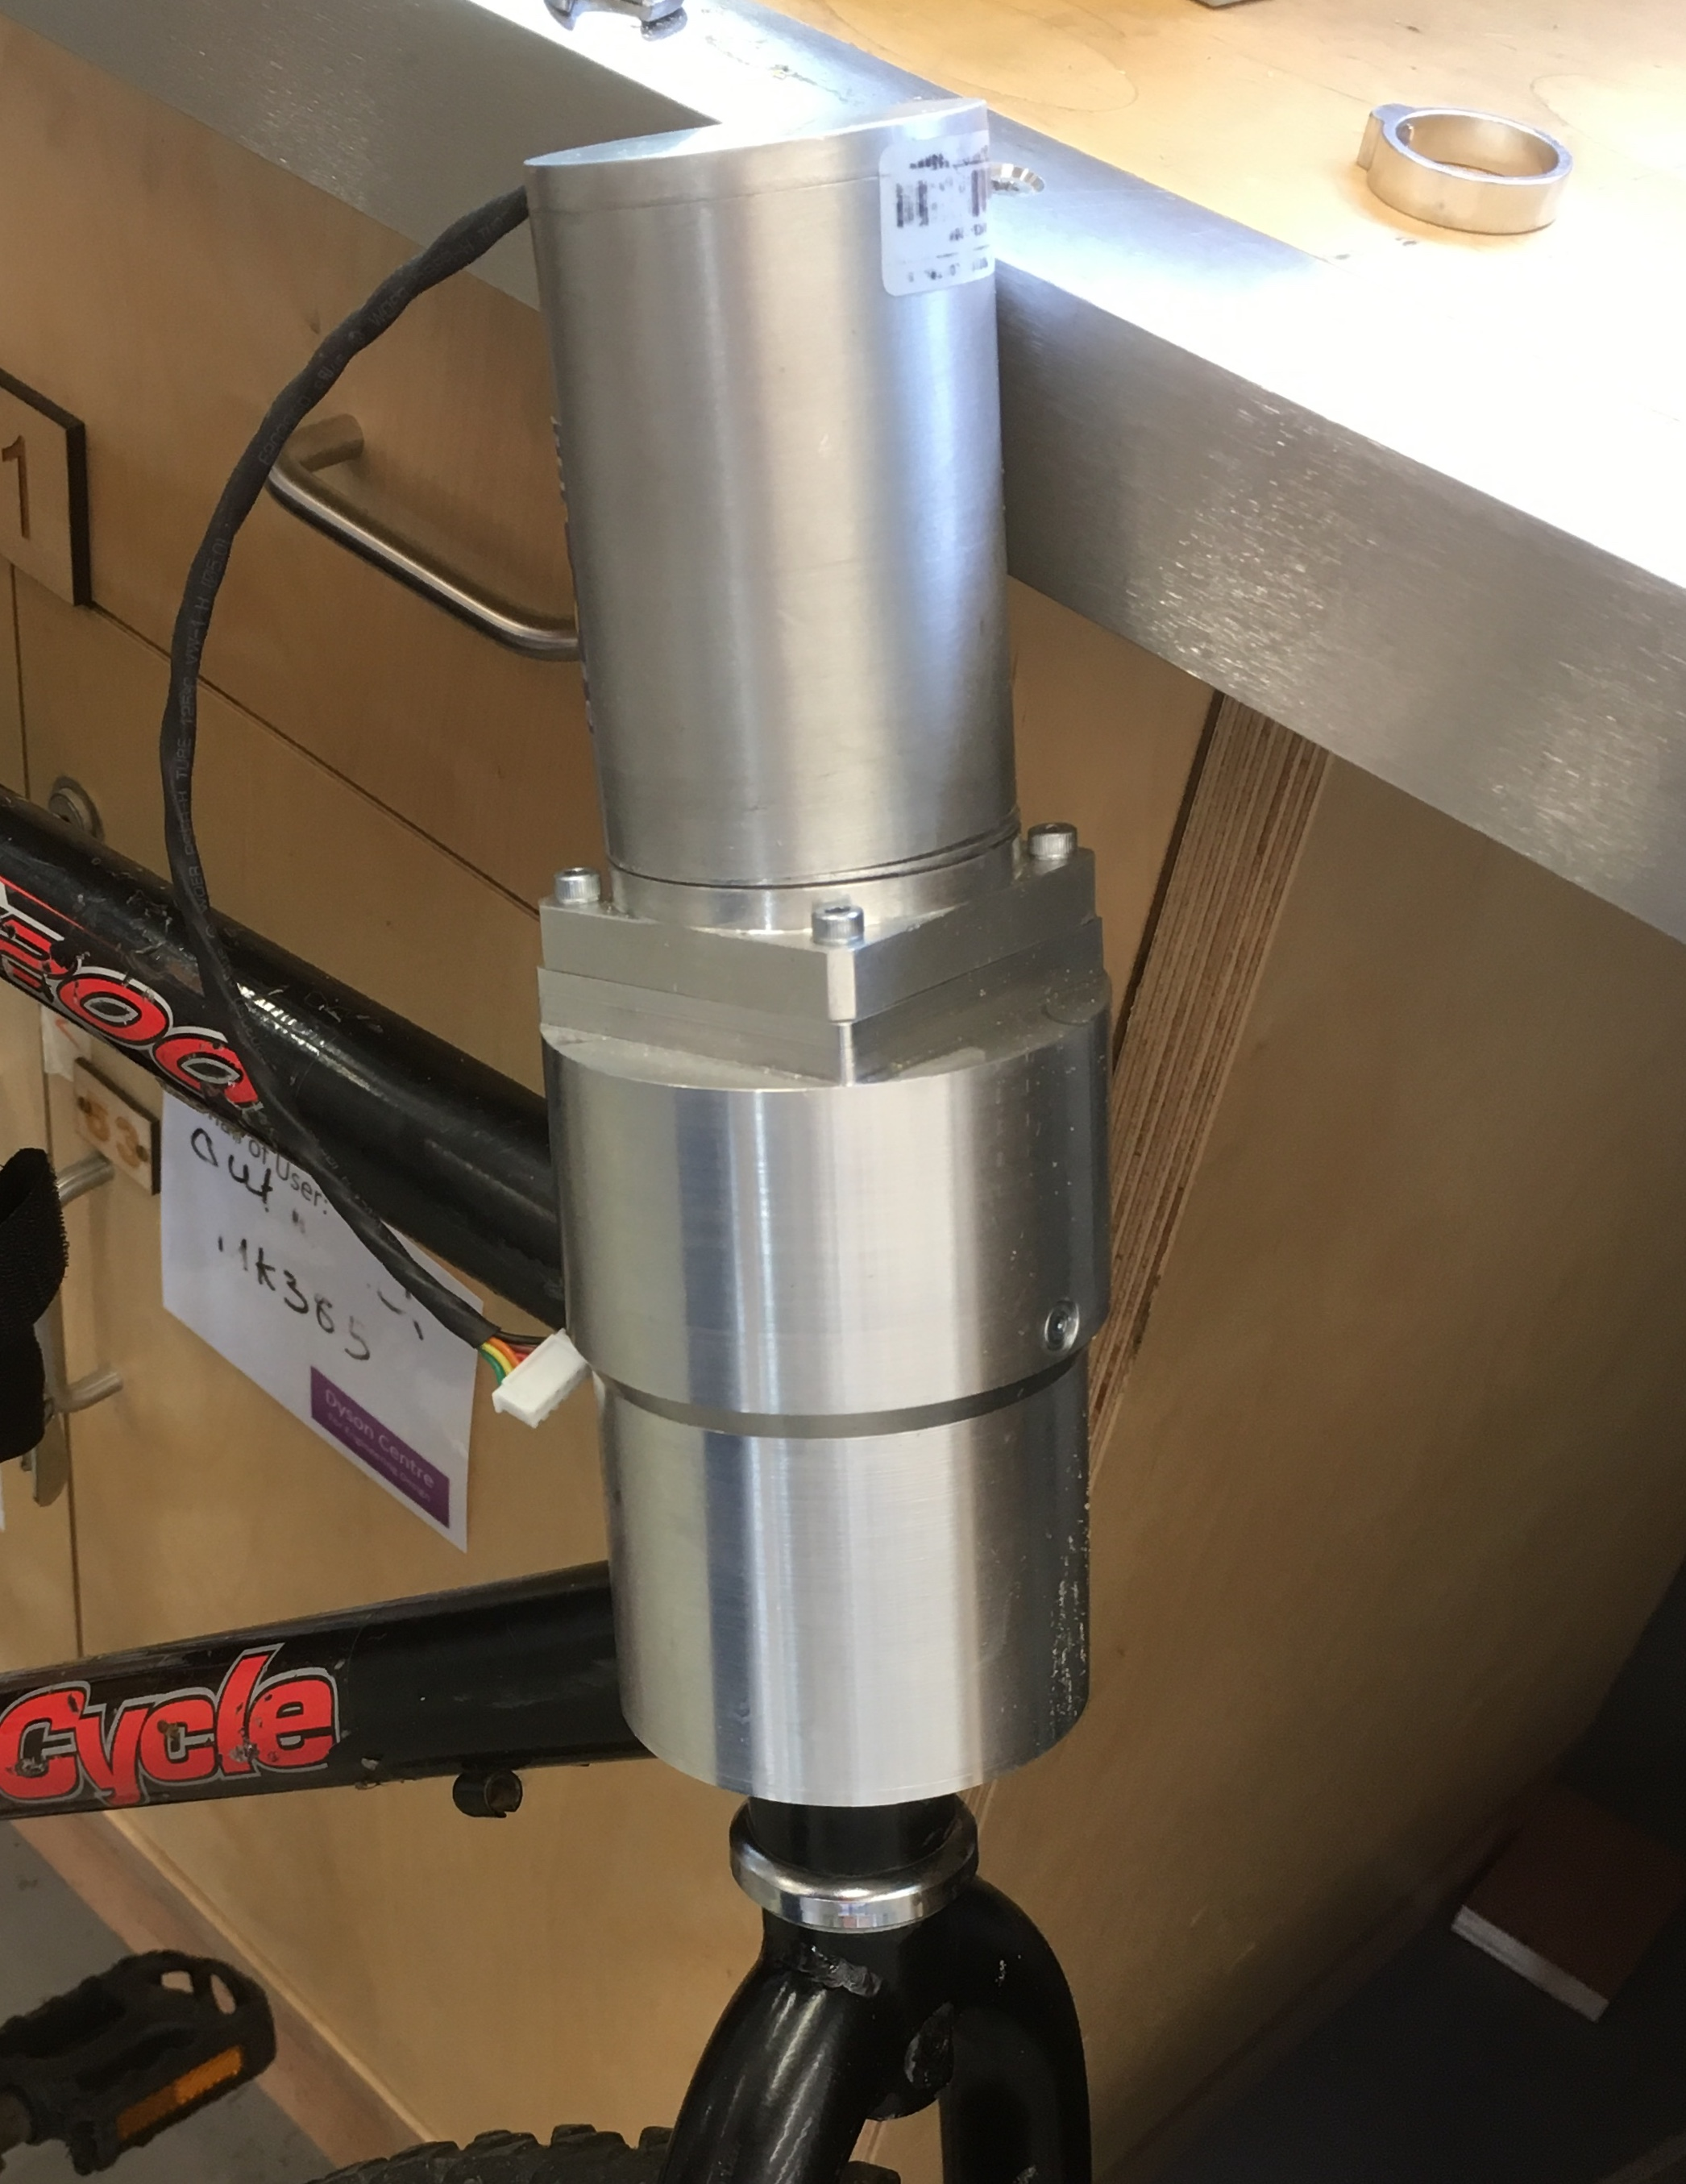
\includegraphics[width=\textwidth]{fsServo}
		\caption{Servo Assembly}
	\end{subfigure}
	\hfill
	\begin{subfigure}[t]{0.475\textwidth}   
		\centering 
		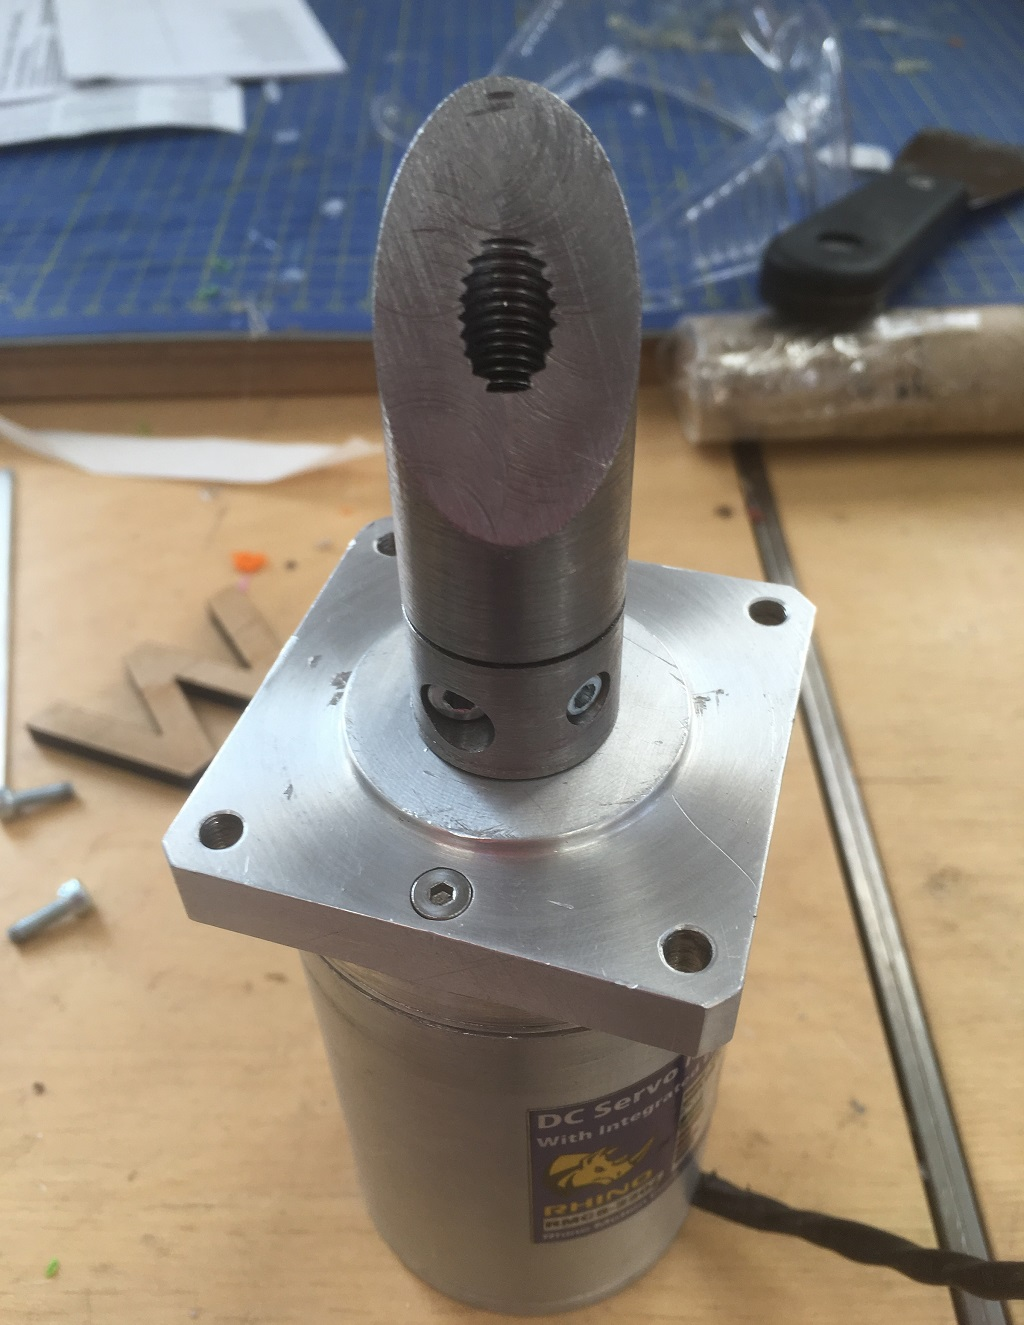
\includegraphics[width=\textwidth]{fsServoMount}
		\caption{Servo Mounting Mechanism}
	\end{subfigure}
	\caption{Full-Scale Bicycle Hardware}
	\label{fig:fsHardware}
\end{figure}
\vfill

\subsection{Software}
The microprocessor was programmed using the C programming language. The software structure was very similar to that developed for the Lego prototype, however with the addition of the following items:

\begin{enumerate}
\item{Remote Control:}
\item{Multiple Timed Loops:}
\item{Inertial Measurement Unit:}
\item{Servo:}
\item{Logging via Radio:}
\end{enumerate}

\subsubsection{Lean Angle Estimation}
Again, it was necessary to estimate the lean angle from raw sensor data. In the case of the full-scale bicycle however, an \textit{inertial measurement unit} (IMU) was available, comprised of three gyroscopic sensors and three accelerometers, each aligned along an orthogonal axis. This meant that gyroscopic drift could now be directly accounted for without having to resort to the computationally expensive Kalman filter used for the Lego prototype.\\

At rest, an accelerometer produces a signal directly proportional to the gravitational vector, this can then be used as a reference to correct for gyroscopic drift. However, when in accelerated motion, the accelerometer output will be \textit{corrupted} by other accelerations terms, such as linear or Coriolis. \\

The problems present in both accelerometers and gyroscopic sensors are alleviated to an extent by the use of a \textit{complementary filter}, for which the corresponding block diagram can be seen in Figure \ref{fig:CF} below. An estimate of the lean angle $\hat{\phi}_a$ is computed using accelerometer measurements and then finally low-pass filtered. This estimate is summed with integral of the high-pass filtered, gyroscopic sensor measurements $\dot{\phi}_g$ to give an improved estimate of the lean angle $\hat{\phi}_{cf}$. The low- and high-pass filters both use the same cut-off frequency given by $1/\tau$. In this way, the stable low-frequency accelerometer data is combined with the drift-free, high-frequency gyroscope data to give an estimation based on multiple, noisy sources.

\begin{figure}[H]
	\centering
    \def\svgwidth{0.5\textwidth}
    \input{./figures/compfilt.pdf_tex}
    \caption{Complementary Filter Block Diagram}
	\label{fig:CF}
\end{figure}

The discretised form of the complementary filter, used in implementation, is given by the following difference equation:
\begin{equation*}
\hat{\phi}_n = \alpha \cdot \hat{\phi}_a + (1 - \alpha) \cdot (\hat{\phi}_{n-1} + \dot{\phi}_g \cdot T)
\end{equation*}

Where the constant $\alpha$ determines the weighting between accelerometer and gyroscope measurements. As $\alpha \rightarrow 0$, the estimate is heavily reliant on gyroscope readings, and as $\alpha \rightarrow 1$, accelerometer estimates are favoured. $\alpha$ is typically chosen to near zero, so that the accelerometer merely acts as a long-term correction factor. \\
Lastly, it is evident that this simple difference equation is computationally far less expensive than the aforementioned Kalman filter.

\subsubsection{Basestation and Telemetry}

\begin{figure}[h]
\centering
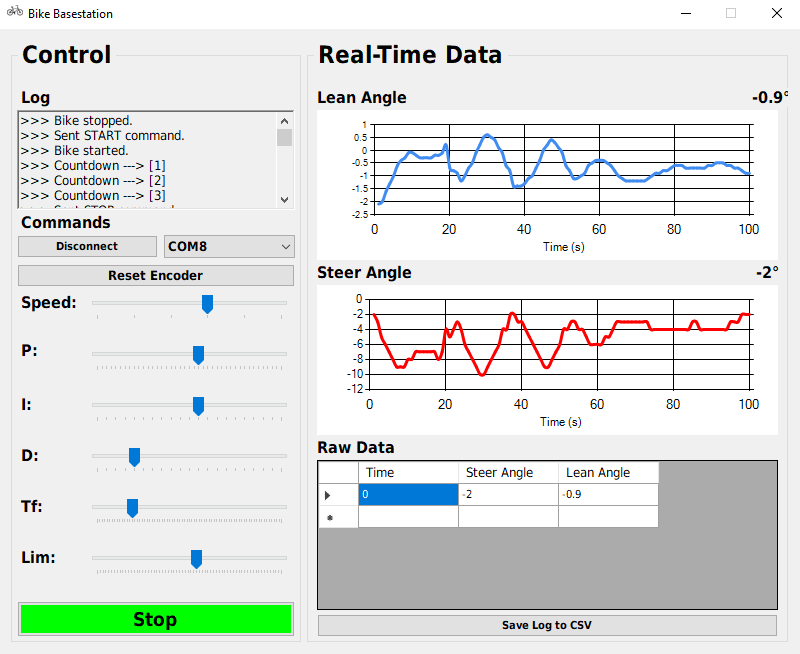
\includegraphics[scale=0.5]{Basestation}
\caption{Screenshot of Bicycle Basestation}
\label{fig:basestation}
\end{figure}

Packet handling, vary controller parameters on the fly, live data logging and display, safety start/stop, etc..

\subsection{Results}